%%%%%%%%%%%%%%%%%%%%%%%%%%%%%%%%%%%%%%%%%
% Stylish Article
% LaTeX Template
% Version 2.1 (1/10/15)
%
% This template has been downloaded from:
% http://www.LaTeXTemplates.com
%
% Original author:
% Mathias Legrand (legrand.mathias@gmail.com) 
% With extensive modifications by:
% Vel (vel@latextemplates.com)
%
% License:
% CC BY-NC-SA 3.0 (http://creativecommons.org/licenses/by-nc-sa/3.0/)
%
%%%%%%%%%%%%%%%%%%%%%%%%%%%%%%%%%%%%%%%%%

%----------------------------------------------------------------------------------------
%	PACKAGES AND OTHER DOCUMENT CONFIGURATIONS
%----------------------------------------------------------------------------------------

\documentclass[fleqn,10pt]{SelfArx} % Document font size and equations flushed left

\usepackage[english]{babel} % Specify a different language here - english by default

\usepackage{graphicx}
\usepackage{caption}
\usepackage{subcaption}
\usepackage{gensymb}

\usepackage{lipsum} % Required to insert dummy text. To be removed otherwise

%----------------------------------------------------------------------------------------
%	COLUMNS
%----------------------------------------------------------------------------------------

\setlength{\columnsep}{0.55cm} % Distance between the two columns of text
\setlength{\fboxrule}{0.75pt} % Width of the border around the abstract

%----------------------------------------------------------------------------------------
%	COLORS
%----------------------------------------------------------------------------------------

\definecolor{color1}{RGB}{0,0,90} % Color of the article title and sections
\definecolor{color2}{RGB}{0,20,20} % Color of the boxes behind the abstract and headings

%----------------------------------------------------------------------------------------
%	HYPERLINKS
%----------------------------------------------------------------------------------------

\usepackage{hyperref} % Required for hyperlinks
\hypersetup{hidelinks,colorlinks,breaklinks=true,urlcolor=color2,citecolor=color1,linkcolor=color1,bookmarksopen=false,pdftitle={Title},pdfauthor={Author}}

%----------------------------------------------------------------------------------------
%	ARTICLE INFORMATION
%----------------------------------------------------------------------------------------

\JournalInfo{Journal, Vol. ..., No. ... 2017} % Journal information
\Archive{Additional note} % Additional notes (e.g. copyright, DOI, review/research article)

\PaperTitle{Foliage detection project} % Article title

\Authors{Iuliia Pliushch\textsuperscript{1}*, Dennis Soukup\textsuperscript{2}*, Wolfgang Stammer\textsuperscript{3}*} % Authors
\affiliation{*\textit{Goethe University, Frankfurt am Main}} % Author affiliation
\affiliation{\textsuperscript{1} ipliush@stud.uni-frankfurt.de} % Corresponding author
\affiliation{\textsuperscript{2} s4811888@stud.uni-frankfurt.de}
\affiliation{\textsuperscript{3} s5401424@stud.uni-frankfurt.de}

\Keywords{contextual models, blender scripting, foliage detection} % Keywords - if you don't want any simply remove all the text between the curly brackets
\newcommand{\keywordname}{Keywords} % Defines the keywords heading name

%----------------------------------------------------------------------------------------
%	ABSTRACT
%----------------------------------------------------------------------------------------

\Abstract{This is the summary of the foliage detection project. The aim is to construct the context model of foliage detection on the ground by means of a drone with a camera, create artificial data with blender scripting on its basis, design an algorithmic pipeline for foliage detection on those artificial images and analyze its performance by relating it to the parameters of the model.}

%----------------------------------------------------------------------------------------

\begin{document}

\flushbottom % Makes all text pages the same height

\maketitle % Print the title and abstract box

\tableofcontents % Print the contents section

\thispagestyle{empty} % Removes page numbering from the first page

%----------------------------------------------------------------------------------------
%	ARTICLE CONTENTS
%----------------------------------------------------------------------------------------

\section*{Introduction} % The \section*{} command stops section numbering

\addcontentsline{toc}{section}{Introduction} % Adds this section to the table of contents

This project focuses on creating a context model of foliage generation and distribution in a private property, generating graphical data based on this model and training a machine learning system to recognize foliage in the generated images. The project thus covers the subject of task specific context and generative modelling, systems design and finally systems engineering. The inspiration for this project was driven by the software engineering class. While the \emph{software} engineering class emphasizes the practical side of the project (flying the drone, gathering real data with it and detecting foliage on its basis), the \emph{systems} engineering class emphasizes the context model creation that should be a preceeding step for the software engineering. The relationship between real and simulated data is more profoundly considered in \cite{Subu:2015}. \\
We begin our project by precisely defining the task and context model parameters. We next create graphical models of the world in order to generate realistic graphical images using blender scripting. Here it is important to note that the images are realistic not based on all world parameters, but only those we assume to be important for foliage generation and distribution and which we assume to lead to important features for algorithmic detection.  We then consider which parameters of the context model provide sufficient amount of information about foliage in order to construct an algorithmic pipeline to create classified images (classified into foliage and non-foliage).

\section{Context model}

\begin{figure*}[ht!]
\begin{enumerate}[nolistsep]
 \item \underline{Task: Foliage detection}:
    \begin{enumerate}[nolistsep]
	\item 2D foliage detection: Detection on the basis of only \textbf{one} picture
	\item 3D reconstruction: Use sequences of 2D images from the flying camera to reconstruct the 3D surface and detect foliage there. Here, camera trajectory is imporant.
	\item \emph{What}: Tree and bush foliage
	\item \emph{Where}: Detection of fallen leaves on the ground
	\item \emph{When}: Real time or not, offline or online
	\item Success criterions: 
	  \begin{enumerate}[nolistsep]
	    \item Detection step (our): Percentage of correctly as belonging to foliage classified pixels. Alternatively one can also take the trade-off between performance and processing time.
	    \item Overall: The ground is cleared from fallen leaves (foliage).
	  \end{enumerate}
    \end{enumerate}
 
 \item \underline{Camera}:
    \begin{enumerate}[nolistsep]
    \item Parameters: pixel resolution, type of lens and focus, saturation, zoom factor, motion blur, lighting type, lens staining (e.g., dependent on weather)
    \item Flying trajectory
    \end{enumerate}
      
  \item \underline{Scene}:
    \begin{enumerate}[nolistsep]
     \item Objects:
	\begin{enumerate}[nolistsep]
	    \item \textbf{Ground}
	      \begin{enumerate}[nolistsep]
		\item Geometric form (if square, its width and breadth; if circle, its radius)
		\item Surface type (e.g., gras vs. asphalt) and properties (leaf-like color or not)
	      \end{enumerate}
	    \item House (we do not consider variation of this object type)
	    \item \textbf{Tree}
	      \begin{enumerate}[nolistsep]
		\item Object properties: tree height, diameter of the tree trunk, diameter and amount of branches, amount and type of leaves, color (different interpolations of colors, except for blue) etc. 
		\item Object location distributions: 
		\begin{itemize}
		    \item single distribution, e.g. Gaussian
		    \item multiple distribution: e.g. trees near the boundaries of the property and right near the house
		\end{itemize}
	    \end{enumerate}
	    \item \textbf{Foliage} (leaves on the ground)
	      \begin{enumerate}[nolistsep]
		\item Object properties: size, geometric form (e.g., curvature of the leaf boundary and curvature of the leaf plane) and structure (leaf skeleton type, symmetry), shadow-rich areas of high contrast \cite{Hamme:2008}, randomness of edges, varying color (yellow-brown-red)
		\item Texture properties: reflection and rough texture
		\item Object location distributions: e.g. Gaussian
	      \end{enumerate}
	\end{enumerate}
    \item Conditions: 
      \begin{enumerate}[nolistsep]
		\item Weather: sunny, rainy, foggy, wind
		\item Time of the day: day, night, sunset, sunrise
		\item Season (time of the year): light intensity, snow
      \end{enumerate}
    \end{enumerate}

\end{enumerate}
\caption{Context model parameters}
\label{fig:context}
\end{figure*}

\subsection{Enlistment of context parameters}
In this section we describe the specific task of our system, the context model parameters and graphical models.\\
\textbf{General setup}: The case that we are exploring here is that of a drone flying over some private property which contains a house, a yard and trees. 

Our context model (see figure \ref{fig:context}) will contain three sets of parameters:

\begin{itemize}
 \item the parameters of the assignment (task) that is to be solved
 \item the parameters of the drone (most importantly parameters of the camera)
 \item the paramters of the (generative) world model
\end{itemize}

Below we will briefly summarize some of the parameters and properties stated in figure \ref{fig:context}.  \\

\textbf{Task}: The task is to detect (and remove) foliage that has fallen from the trees, in other words, fallen leaves. We will restrict our summary and analysis to the subtask of fallen leaves detection, not removal. As input for this subtask, one can take either a single image or a sequence of images generated at certain time intervals at different angles. Our success criterion is the percentage of correctly classified pixels.

\textbf{Drone/Camera}: The drone contains a camera with preset parameters and can change its flying trajectory. 

\textbf{World: Ground properties}: We consider a plane with different textures and colors, for example a combination of grass and asphalt.

\textbf{World: Tree properties}: Several properties of trees vary depending on the time of the year, for example the amount of leaves, their color etc. Others depend on the tree type, for example the diameter of the tree trunk.

\textbf{World: Tree location}: Tree location may stem from different combinations of distributions. Natural tree location can be approximated with a Gaussian distribution, but man-made gardens may also contain regularities, such as planting the tree at the outer boundary of the property and near the house.

\textbf{World: Leaf properties}: Leaf properties may vary depending on the tree type, e.g. size, structure, geometric form. Others may depend on the time of the year, e.g. color. Groups of leaves build together shadow-rich areas. Leaves are symmetric and contain a periodic skeleton.

\textbf{World: Leaf location}: Leaves can fall off the trees and, hence, distribute over the property such that right below the tree the amount of leaves from that tree will be greater than further away. One possibility is to assume that leaves are Gaussian distributed with respect to the trees that they fall off. This may be influenced by weather conditions, such as wind which would cause scattering of the leaves if strong enough.

\textbf{Conditions} Light conditions can be influenced by the weather and season of the scene, e.g. the light intensity and angle of the sun. Other weather conditions may influence some properties of leaves listed above, e.g. long dry intervals may create a crumbling effect of the leaves, rain may create reflection of the light from the leaves.

\subsection{Leaf modelling}

\begin{figure}[ht]\centering
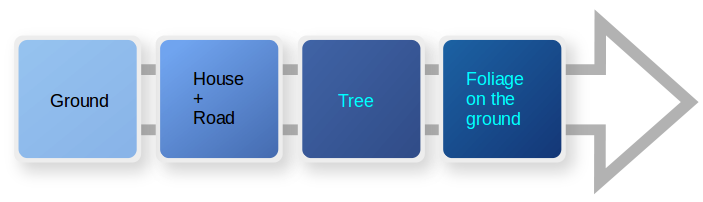
\includegraphics[width=\linewidth]{Figures/sceneObj.png}
\caption{Scene objects}
\label{fig:sceneObj}
\end{figure}

Modelling the scene objects would need to start with choosing the \emph{location} and \emph{properties} of the ground, then doing the same for the house, road, trees and, lastly, leaves (see figure \ref{fig:sceneObj}). The location and properties of the scene object that is constructed first, constrain all the other objects generated later. This is because, given the constraint of where the house is located and how big it is (a property of the house), the trees could not be at the same position as the house.

\begin{figure}[ht]\centering
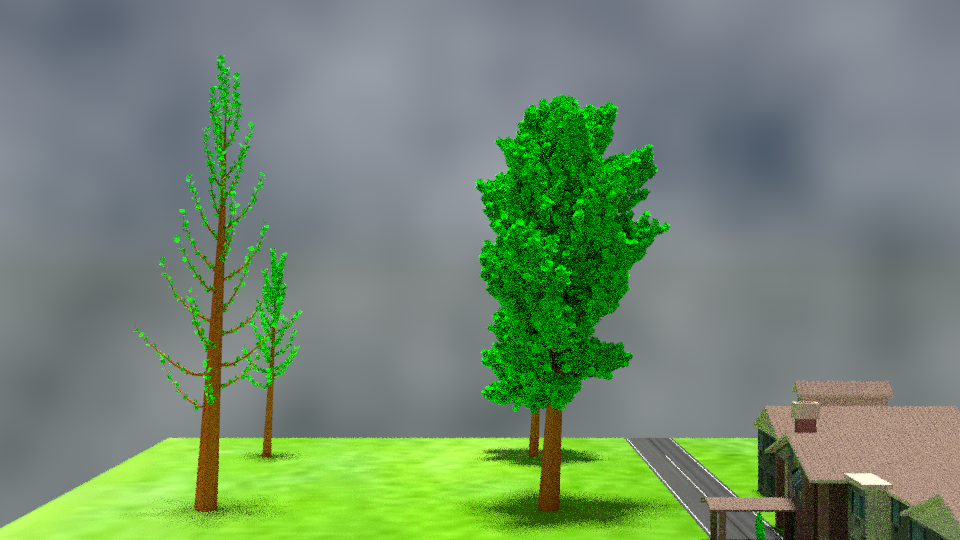
\includegraphics[width=\linewidth]{Figures/ex1.png}
\caption{Blender Sapling Add-on}
\label{fig:sapling}
\end{figure}

\subsubsection{Foliage distribution on the ground}

Let us start modelling the \emph{location} and the \emph{attributes} of fallen leaves, because they are the most important scene object, in the light of the foliage recognition task. For tree modelling, an already existing Sapling Add-on of Blender can be used, see \ref{fig:sapling}.  As for the distribution of the location of the leaves, a \emph{spatial stochastic point process} can be used. It may be described such that the ground is dissected into subparts (e.g. a grid), for each of which a probability of falling leaves can be assigned according to a certain distribution. In the case of leaves, a bivariate (2D) mixture of Gaussians (see \ref{fig:gausMix}) builds a good starting point for describing such a distribution. 

\begin{figure}[ht]\centering
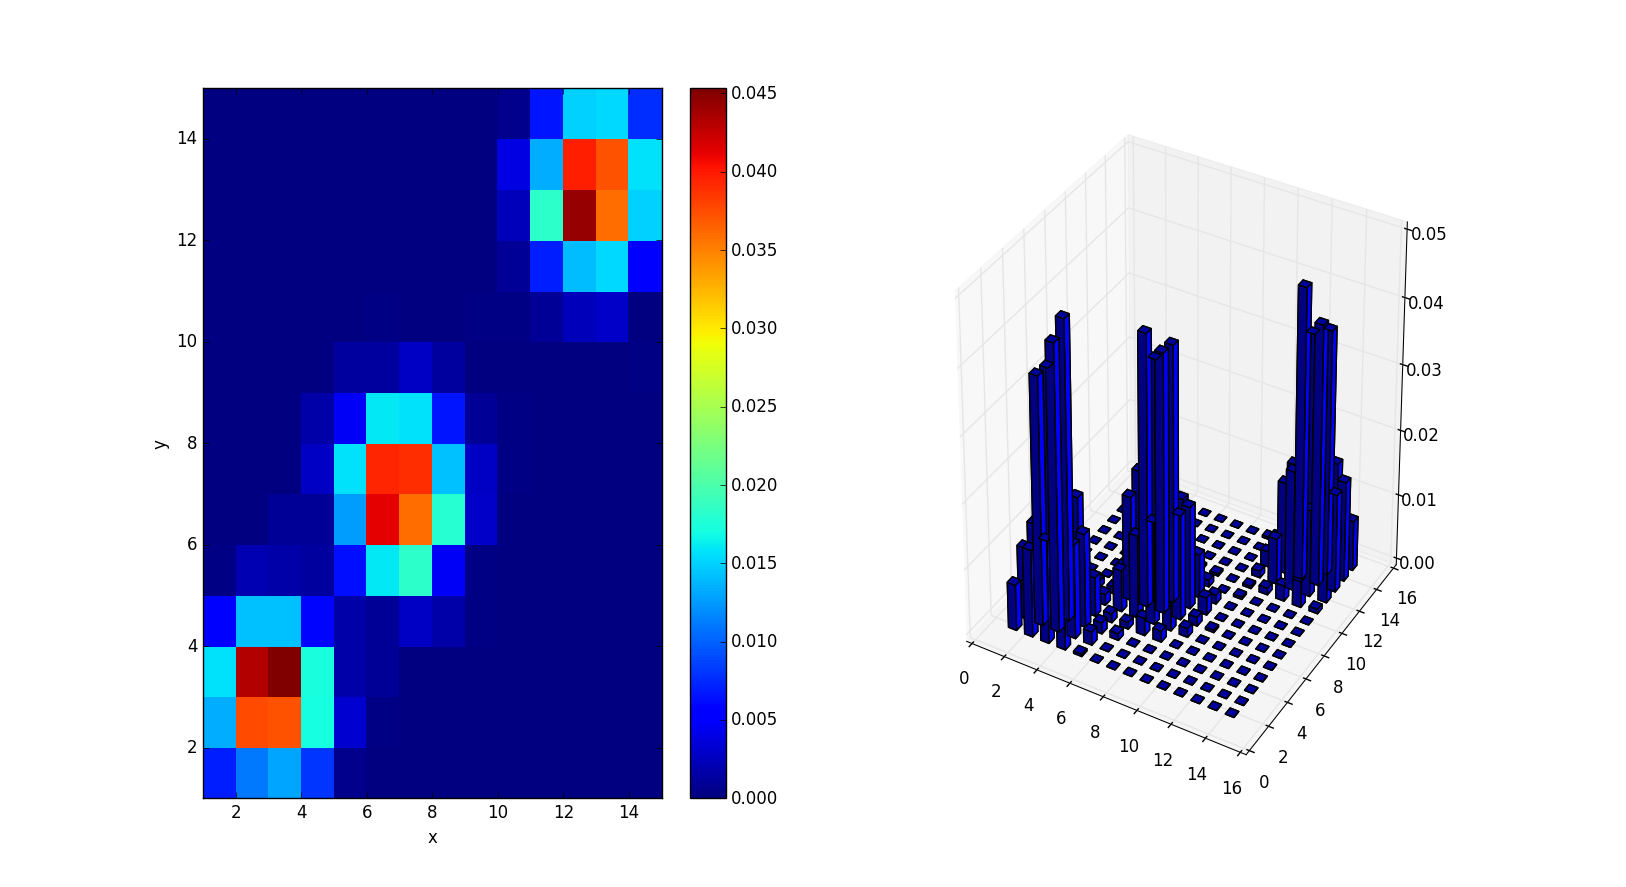
\includegraphics[width=\linewidth]{Figures/gausMix.png}
\caption{Bivariate mixture of Gaussians with three trees: Plot of fallen leaf samples for given $\delta$ x and $\delta$ y}
\label{fig:gausMix}
\end{figure}

Given the position of trees, the distribution of foliage on the ground would be a (modified) bivariate (2D) mixture of Gaussians with the \emph{means} of those Gaussians being determined by the locations of the trees and the \emph{(co-)variances} by the weather conditions (e.g. high variance when it is windy) and topological constrains (e.g., leaves gathering near fences or outer walls of houses), see figure \ref{fig:leafLoc}. The modification of this probability distribution is needed, because though leaves are more often found under the tree, than far away from it, the proximity to the tree is bounded by the tree trunk radius. In other words, there will be no fallen leaves \emph{inside} the tree. Figure \ref{fig:gausMixSinus} shows one such weighting possibility by means of a sinus: $a_{i}$, as well as the \emph{variance} of the Gaussian component are varied such that one can model, respectively, different sizes of the tree trunk and different amounts of leaves that one tree has.

The amount of leaves that are sampled from the distribution of a single tree depends on the initial amount of leaves on the tree, conditioned on the tree type, and the time of the year.

\begin{figure}[ht]\centering
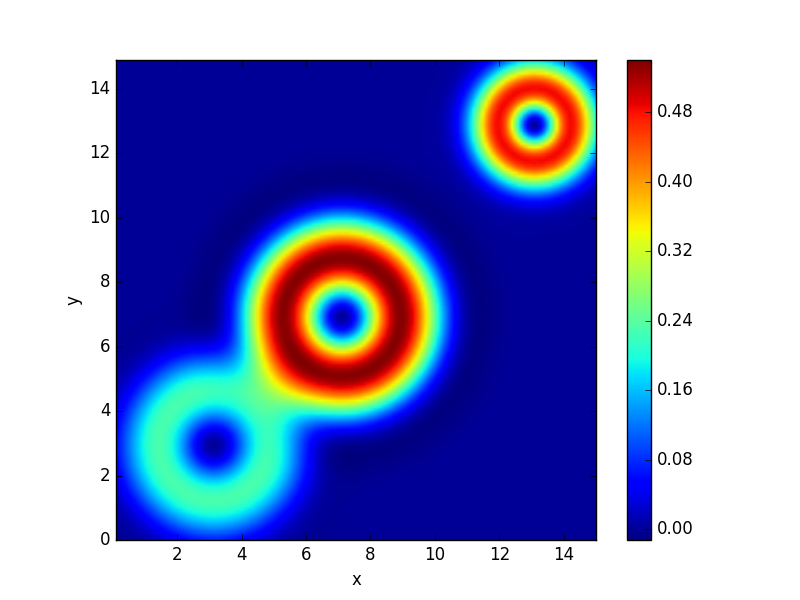
\includegraphics[width=\linewidth]{Figures/gausMixSinus.png}
\caption{Bivariate mixture of Gaussians, where each component is weighted by $a_{i}*k*sin((mean_{i}-x)^{2}+(mean_{i}-y)^{2})$ with $k=0.2$}
\label{fig:gausMixSinus}
\end{figure}

\begin{figure*}[!ht]\centering
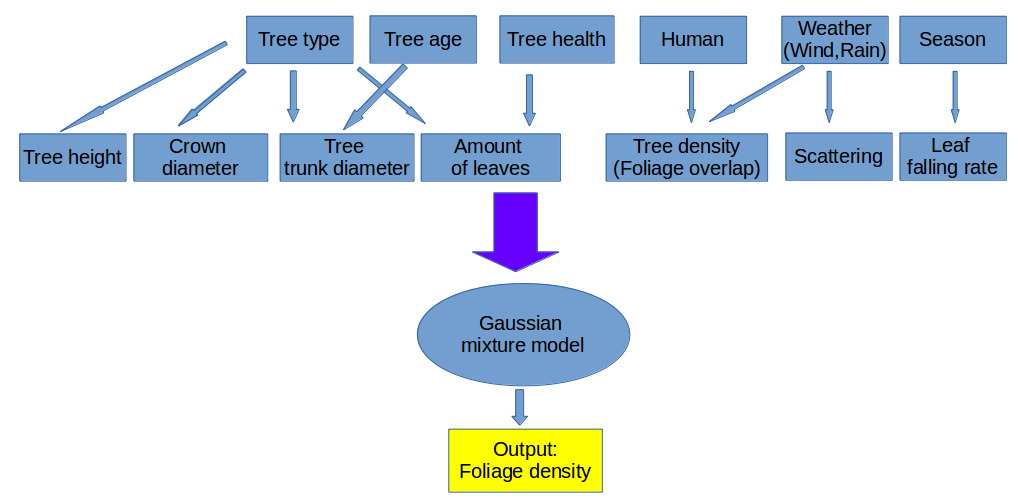
\includegraphics[width=0.8\linewidth]{Figures/leafLoc.png}
\caption{Main parameters contributing to the Bayesian model of foliage location}
\label{fig:leafLoc}
\end{figure*}

\subsubsection{Foliage and leaf geometry}

Depending on foliage density, leaves may be scattered or clustered, see \ref{fig:leafFoliage}. Therefore, it is necessary to distinguish between the geometry of a single leaf and clustered leaves. 

\begin{figure}[ht]\centering
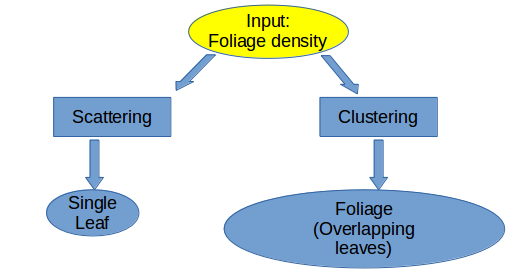
\includegraphics[width=\linewidth]{Figures/leafFoliage.png}
\caption{Foliage geometry as a result of either scattering or clustering}
\label{fig:leafFoliage}
\end{figure}

Regarding leaf properties, one can distinguish between their \emph{geometry}, as well as \emph{texture} properties. Since our task is to detect several leaves, the fact that fallen leaves may \emph{overlap} will also come into play. In \cite{Kumar:2012}, the distinctive shape of leaves is used as a sole recognition cue for categorizing them (establishing their type). This is because their color or venation pattern are too variable. Leaf color varies depending on the season and weather conditions. The venation pattern is visible only when the resolution of the camera is good, see \ref{fig:leafGeom}.

\begin{figure}[ht]\centering
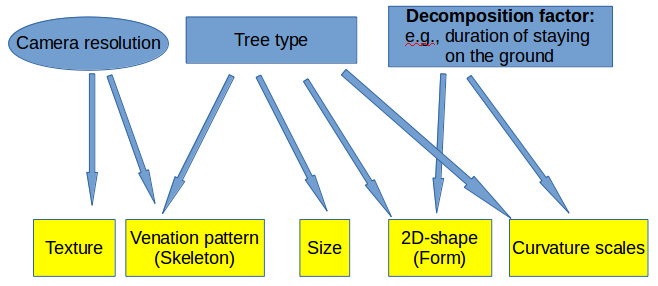
\includegraphics[width=\linewidth]{Figures/leafGeom.png}
\caption{Main parameters contributing to the Bayesian model of leaf geometry and texture}
\label{fig:leafGeom}
\end{figure}

The geometrical and textural properties of a single leaf are described in figure \ref{fig:leafGeom}. The geometrical and textural properties of foliage include:

\begin{itemize}[nolistsep]
 \item random edges/high variance of edge directions
 \item minimum edge density
 \item a shadow-rich area
\end{itemize}

Given that there are at least two ways, in which one might represent foliage: either as a \emph{curved surface}, or as a \emph{point cloud}, we have, in agreement with \cite{Kumar:2012},  decided to use the second option, because leaves may consist of smaller components or clusters (e.g. pine needles), such that the curvature would be difficult to compute. From the point cloud, the leaf contour as an "array of contiguous point locations" can be computed and the scale-dependent leaf curvature can be subsequently extracted, see \cite{Kumar:2012}.

\subsubsection{Foliage photometry}

Photometry is influenced by motion blur (1), illumination (2) and specular reflection (3), while foliage color distribution depends on the latter two,  see \ref{fig:foliagePhotometry}. Importantly, the leaf color changes with the time of the year (season). Finally, weather can increase or decrease the amount of specular reflection.

\begin{figure}[ht]\centering
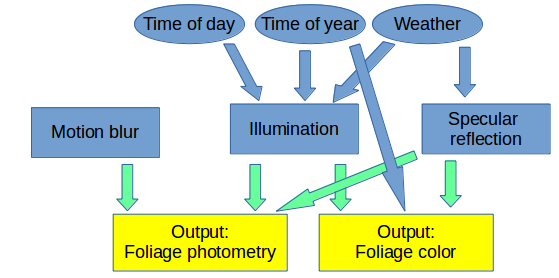
\includegraphics[width=\linewidth]{Figures/foliagePhotometry.png}
\caption{Main parameters contributing to the Bayesian model of foliage photometry}
\label{fig:foliagePhotometry}
\end{figure}

\section{Realization of the model in Blender}

Though our graphical models are already a simplification, we further simplify them for our foliage recognition task. This is because we assume that some parameters are more important than others for foliage recognition. We hypothesize that important leaf detection features are leaf form/geometry, leaf location (namely on the ground and not on the trees), color distinction with respect to background, sufficient amount of random edges and shadow-rich areas. Thus, we vary only those parameters in our graphical models that are most important for the mentioned detection features. Here we mainly focused on the parameters determining the construction and location of individual leaves. Such other parameters of our model as, for example, "tree health" and "tree age" have been ignored. As for "tree type", we have introduced randomization into some tree parameters, as the number of branches and the trunk diameter. Nevertheless, those randomized parameters do not necessarily coincide with a certain real tree type. 

\subsection{Simplification of graphical model parameters}

Following parameters of our graphical models we have further simplified or excluded:
 
\textbf{Tree location}: Instead of modelling a complex arranging of trees on the property, as a first step we use only fixed positions.

\textbf{Tree type}: As described above we randomly produce trees by randomly varying the parameters of the sapling add-on add\_tree() function. Thus every tree looks different and has individual parameter values, but these do not correspond to real tree types.
 
\textbf{Tree age, Tree health, Season}: These parameters were ignored entirely in the blender scripting.
  
\textbf{Amount of leaves}: The parameter "Amount of leaves", similarly as "Tree type" we have modelled by randomly varying the tree parameters in the add\_tree() function. That is we do not vary this conditioned on the season.
 
\textbf{Leaf falling rate}: This is modelled as a gaussian distribution without considering the time of year. 

\subsection{Leaf geometry}

In order to keep the geometry and form of leaves as realistic as possible we have chosen to model leaf geometry by using photographs of five different kind of leaves, loading them in Blender and changing their color. This way, we can benefit from the realistic leaf form and texture. Furthermore, the geometric object to which we add the leaf texture is a grid. We randomly add noise to grid points such that our leaf is not a pure 2D plane, but a randomly \emph{bent} one, see \ref{fig:leaf_bend}. 

\begin{figure}[ht]\centering
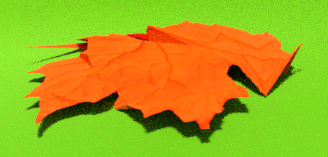
\includegraphics[width=\linewidth]{Figures/leaf_bend.png}
\caption{Single leaf}
\label{fig:leaf_bend}
\end{figure}

This way not only bending, but also crumbling of leaves can be realized, if the noise degree is sufficiently high. We assign to each tree a leaf type, so that the distribution of leaves looks realistic.

\subsection{Leaf distribution}

We have simplified the distribution we have described previously such that for each tree, we sample from a multivariate gaussian with the tree location as our mean, but instead of the sinusoidal function to push the leaves out of the tree trunk we just sample x,y positions outside of the trunk diameter and within the property boundaries. Scattering of the leaves, for example by wind, we model by varying the variance and covariance of the multivariate distribution.

\begin{figure}[ht]\centering
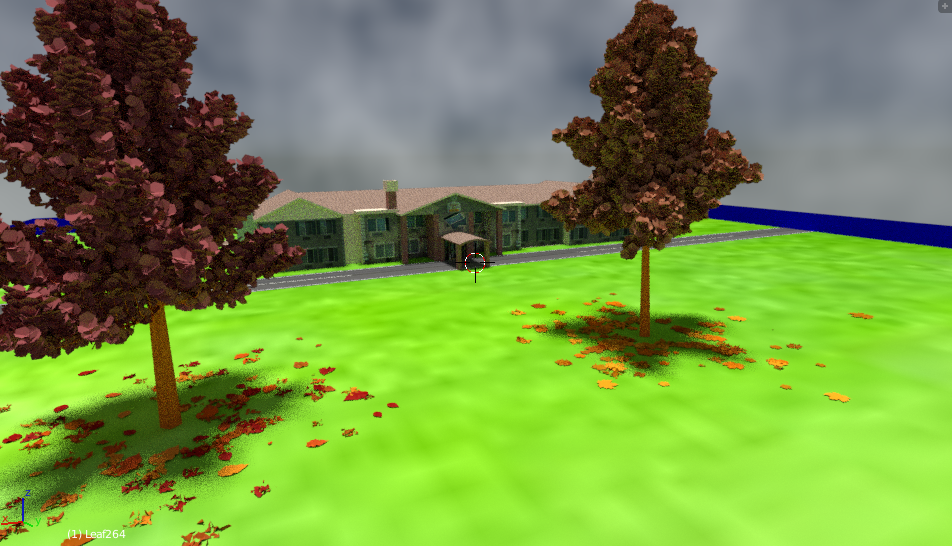
\includegraphics[width=\linewidth]{Figures/trees.png}
\caption{Coloured tree leaves}
\label{fig:trees}
\end{figure}

\subsection{Tree geometry}

The tree parameters that we manipulate during tree generation with the Sapling Add-on are:

\begin{enumerate}[nolistsep]
 \item tree trunk diameter
 \item tree height
 \item number of branches
 \item number and color of fallen leaves
\end{enumerate}

We model the parameters above by means of normal and uniform distribution. 

Our assumption is that for our task it is not important that leaves on the trees and on the ground have the same geometric form and texture. We use the predefined geometric leaf shape from Sapling for the trees, but use a realistic form for the leaves on the ground.

\begin{figure}[ht]
\begin{enumerate}[nolistsep]
	\item \textbf{scene geometry} 
	\begin{itemize}
		\item background: \textit{medium entropy}
		\item ground plane: \textit{low entropy}
	\end{itemize}
	\item \textbf{scene material}: \textit{medium - high entropy}
	\item \textbf{leaf geometry}
	\begin{itemize}
		\item size: \textit{low entropy}
		\item color: \textit{low - medium entropy}
		\item form: \textit{low - medium entropy}
		\item texture: \textit{medium entropy}
	\end{itemize}
	\item \textbf{leaf material}: \textit{medium entropy}
	\item \textbf{environment}
	\begin{itemize}
		\item illumination: \textit{high entropy}
		\item weather: \textit{high entropy}
	\end{itemize}
	\item \textbf{camera geometry}
	\begin{itemize}
		\item position: \textit{low - medium entropy}
		\item internal parameters: \textit{low entropy}
	\end{itemize}
	\item \textbf{camera photometry}
	\begin{itemize}
		\item noise model: \textit{low entropy}
		\item transfer function: \textit{low entropy}
	\end{itemize}
	
\end{enumerate}
\caption{Hypothesized information content of the context variables for the detection task described using entropy.}
\label{fig:InformationContent}
\end{figure}

\subsection{Color adjustment}
We adjust the color of the leaves on the tree to the color of the leaves on the ground, see \ref{fig:trees}. For this, we randomly sample from a several fixed rgb values and slightly vary these for every leaf and tree. 

\section{Algorithmic pipeline}

The next step in our project is to design a pipeline of filters and image transformations that can sufficiently well detect the foliage in our data sets. Again the task is a classification task and the performance metric is the number of correctly labeled pixels using binary values of whether a pixel belongs to foliage or not.

We began by trying out different texture, edge and color filters. However, in order to design an appropriate pipeline for our special task we went back to our context model and the variables that influence our scenes. We analysed these concerning how much information they give to the task. In other words we tried to figure out which of these variables our classifier should be invariant to and which give an ample amount of information to confine the feature space an image lives in.

We thus categorized the scene variables into the categories scene geometry, scene material, leaf geometry, leaf material, camera geometry and camera photometry. These categories were further subdivided and finally given the labels low, medium or high entropy, representing how much information the variable gives to the classification task. 
These results can be seen in figure \ref{fig:InformationContent}.

From this table we can summarize that the background, scene material and environment variables (i.e. illumination and weather) have a high entropy. For example what the house on the property looks like is entirely independent of the foliage classification. Our classifier should also, as another example, be able to detect foliage no matter the type or intensity of illumination. Thus our classifier should be invariant to the variables of these three mentioned categories. This can be achieved by transforming input into a feature space in which highly varying parameters are invariant.

From the table we can, however, also summarize those variables with hypothesized low entropy. In comparison to those with high entropy we can try to use information from these variables to aid our classifier. As an example knowing that an object lies on the ground plane gives us quite a lot of information on whether that object might be a leaf or not. Altogether the categories and variables with low entropy can be described as sensor, leaf size, leaf color, leaf form and ground plane, where camera geometry and photometry variables have been summarized into the category sensor.

That variables of the sensor have low entropy essentially means that there is low amount of noise or variation due to camera settings etc. and that the objects portrayed over several images are portrayed as they are. This can be used as a baseline assumption that in fact the images correctly capture the scene with consistency across all images and few artifacts.

\begin{figure*}[ht]\centering
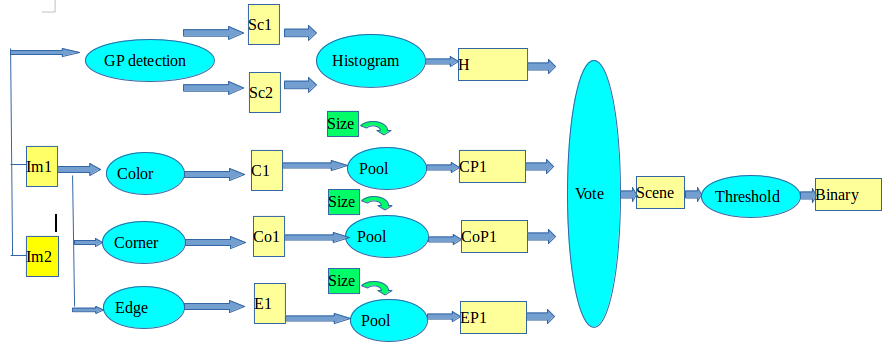
\includegraphics[width=\linewidth]{Figures/PipelineDetail.png}
\caption{Rough pipeline}
\label{fig:Pipeline}
\end{figure*}

The other four variables previously listed with low entropy we can now use for building a pipeline. As a side remark these four variables are very close to the important leaf detection features described in section 2. Further noting that leaf size has a lower entropy than leaf color or leaf form we have designed a rough analysis pipeline depicted in figure \ref{fig:Pipeline}. 

%The ground plane detection is first applied to give a reasonable region of interest (ROI) by excluding all background and objects pointing out vertically from the property, such as trees. The leaf form category described in figure \ref{fig:InformationContent} is divided into orientation of edges and corner edges. As in section 2 we had hypothesized that leaves share a larger amount of corners and randomly oriented edges than other objects or the ground material. 

\subsection{Initial pipeline version}

We began building our pipeline by examining ground plane detection algorithms, leaf color filters and leaf form filters in form of edge and corner detection. The results of this can be found below.

\subsubsection{Ground plane detection}

Our ground plane detection algorithm accepts an image pair (a destination and source image) as input. We apply local feature detection on both images via SURF. The detected features are matched with Flann based matching such that if enough good matches are found the destination image is warped to match the source image (homography). Afterwards the source image is subtracted from the warped image. \\
To turn the resulting grayscale image into a binary image the following filters are applied: median blur $\rightarrow $ erosion $\rightarrow $ binary threshold $\rightarrow$ dilation $\rightarrow $ canny edge detection. Median blur and erosion are applied to get rid of noise grain. To enhance the color value of certain pixels we used a binary threshold of 50. Dilation is applied in order to cancel out the effect of erosion. And finally the canny edge detection is applied to achieve better visualization of the result. Example figures for the filter pipeline can be seen in figure \ref{fig:GroundPlFilt}. \\
 The resulting edges are mapped onto the color source image to visualize the result. An example image for the general algorithm is in figure \ref{fig:GroundPl}.\\

\subsubsection{Leaf color detection} 
 
The color detection procedure is as follows: first, the rgb values of the image are normalized by transposition into the chromaticity space ($\frac{r}{r+g+b}$). Then, on the assumption that leaves on the ground are redder, than greenish or blue, the median filter is applied to the normalized r values. This filter acts as an averager: the pixel value of the most values around it is chosen. The size of the mask should correspond to the size of the leaves here. This filter is used in order to close the gap inside the leaves, with other words, to smooth the foliage area. A threshold can then be set and all pixels above it can be labelled as foliage. As one can see in figure \ref{fig:ColFilters}, the results are reasonable, but sensitive to the magnitude of the threshold. Thus, it might be difficult to choose a threshold that will work equally good on all images.

\subsubsection{Leaf form analysis}

We begin by sliding a rectangular window of the approximate size of a leaf over the original grayscale image. On these so called tiles, we perform a FAST corner edge detection, a canny edge detection, a histogram of gradients and an edge orientation detection. The motivation behind using these filters was the assumption that foliage shows a large amount of different edge orientations and corners. Furthermore we assumed that foliage has a large amount of edges on a small surface area. \\
The results of this step can be found in figure \ref{fig:EdgeFilters} for an example tile in which the filters worked sufficiently well, however many images did not result in such clear leaf edges. However here it can also be seen that also the background material has many different edge orientations (figure \ref{fig:EdgeOrientTile}), if not more than a single leaf does. The corner detection in figure \ref{fig:CornerTile} finds more corners in the noisy background material than in the leaf structure. Canny edge filters (figure \ref{fig:CannyTile}) generate interesting results, however it is not clear how even in this good example the resulting feature map can be used in combination with the results of the previously expressed steps.\\
\begin{figure}[ht]\centering
\includegraphics[width=\linewidth]{Figures/EdgeFigures/EdgeDetectionLeaf.png}
\caption{Final Edge filter example.}
\label{fig:ExEdgeDet}
\end{figure}
Finally better performance was achieved with FAST corner and canny edge filters, if a gaussian filter was first applied to the image. This way some of the noise in the ground texture could be smoothed and reduced. Also small noise in the leaf structure itself could be reduced such that more complete leaf contours were detected. An example can be seen in figure \ref{fig:ExEdgeDet} where starting from the top left to bottom right one can see the original gray scale tile, the canny edge filter results on this tile, the gaussian smoothed tile and finally the edge filter results on the gaussian smoothed tile. 

%Let us consider possible algorithms for foliage detection on the basis of the context model. A characteristic of (dead) foliage that is necessary, but not sufficient, for discrimination is the color. As for foliage that is still on the tree, its green color has been used as a sufficient criterion for detection, see \cite{Berenstein:2010}. Yet dead leaves on the ground exhibit a greater variety in color than leaves on the tree.

%If one were to classify foliage on the trees, one may focus on the randomness of edges characteristic of leaves instead and use color only as an additional criterion. Filters designed for finding local periodic patterns, such as Gabor filters, are ill-suited because of the randomness of the edges distribution in leaves on the trees \cite{Hamme:2008}. The strategy that has been used for foliage detection on the trees in \cite{Hamme:2008} instead is:

%\begin{enumerate}[nolistsep]
 %\item exclude flat, edgeless areas (excludes sky and some man-made objects)
 %\item check for the presence of edges in multiple orientations (due to randomness in the structure of foliage)
 %\item check for the presence of subregions with strong responses (due to shadow-rich zones of foliage with high contrast)
 %\item leaf's color
%\end{enumerate}

%Importantly, filters applied will work better if their size reflects the size of the leaves \cite{Hamme:2008}. But note, that the size of the leaves may vary greatly, depending on the type of trees that one has in the garden.
\section{Performance analysis}

In order to analyse the performance of our pipeline we semantically label the test images, by setting all pixels to certain fixed RGB value corresponding to foliage objects, ground objects and the rest. This can be seen in figure \ref{fig:ExImGT}. This ground truth image we can use to compare how many pixels in our resulting image are correctly labelled as foliage.

\begin{figure}[ht]\centering
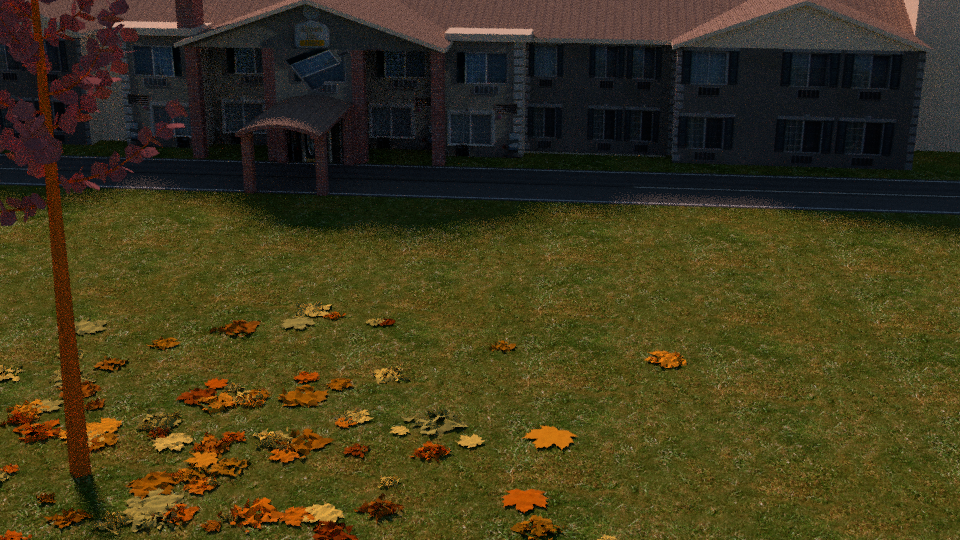
\includegraphics[width=0.45\linewidth]{Figures/im50001.png}
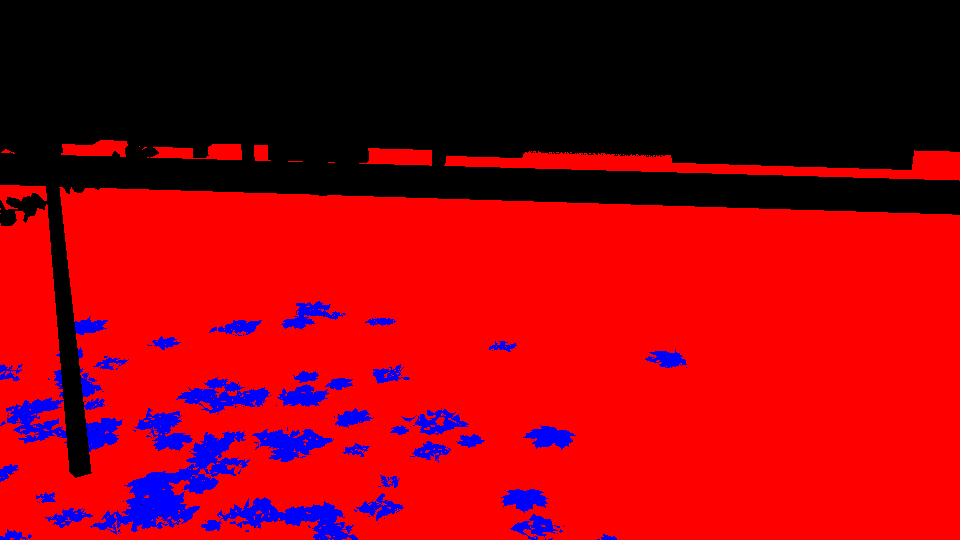
\includegraphics[width=0.45\linewidth]{Figures/im_anno50001.png}
\caption{Semantic labelling of example image used to produce the ground truth labelling.}
\label{fig:ExImGT}
\end{figure}


\section{Results}

From our pipeline, illustrated in figure \ref{fig:Pipeline}, we receive four different feature maps from the modules ground plane detection, color transformation, edge and corner detection. These feature maps we then linearly combine to a single feature map which is thresholded to get a binary classification of foliage vs non-foliage. This binary image we finally compare to the binary ground truth image described above. Exemplary results of our computations can be seen in figure \ref{fig:Res}. 

As can be seen in figure \ref{fig:ResSum}, using all four feature maps did not achieve good results. We noticed that the ground texture (stones) has far too many edges and corners on the scale of the foliage that this could be used for discrimination. Additionally although stated above that the leaf form has low entropy for our task, this in fact is not true given that we allow strong crumbling of the ground leaves, resulting in partly very random leaf forms. Also through the crumbling effect leaves can partly be split thus also changing the size of the leaf.

However using only color transformations and ground plane detection achieved greatly improved results. On the particular image used in figure \ref{fig:Res} and a threshold of $-0.4$ our pipeline correctly detected about 50\% of foliage pixels. We created a dataset with five different ground textures (two grass textures and three sand/stone textures), 50 pictures a texture. Our results can be seen in table \ref{fig:Final}.

We computed four different scores to evaluate our results: accuracy, false positive and false negative rate, as well as $\frac{\text{true positives}}{\text{num of foliage pixels}}$. We also included the number of images, for which the ground detection could not be computed because of the low number of matches. As can be seen, the true positive rate is quite low, but surprisingly consistent over different textures. The false positive rate is very low, but the false negative rate is very high, which means that the color threshold is probably set too high.

\begin{figure}[ht]\centering
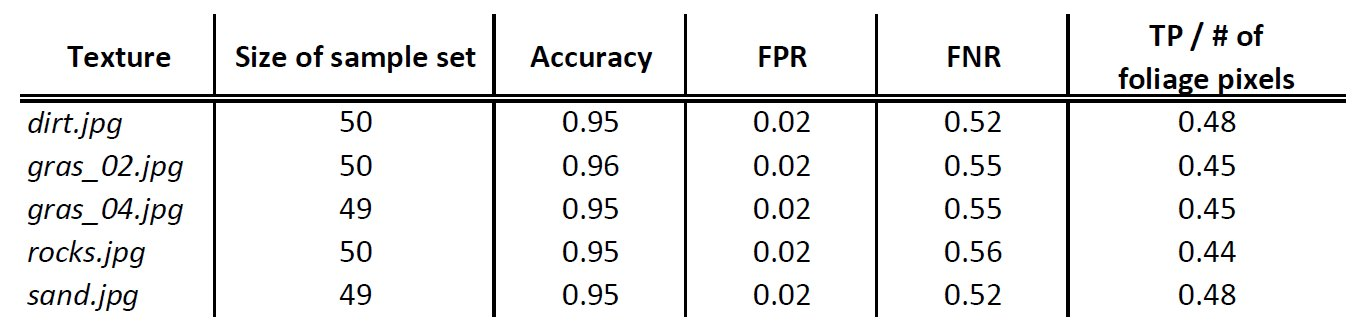
\includegraphics[width=0.95\linewidth]{Figures/table_results.jpg}
\caption{Final results}
\label{fig:Final}
\end{figure}

\section{Discussion}

The color invariant property of foliage could be handled more easily than ground or leaf edge/corner detection. Particularly, bringing the results of edge/corner detection into such a form such that they can be compared to color detection results, was more difficult than expected. 

For future work and improvements it would be worthwhile to improve the ground plan detection. This does not perform as well as it could, such that still many leaves in trees are considered foliage. Also to achieve better results a future task could be to create more complex leaf form filters. Finally, as mentioned above we could try adjusting the final threshold in order to increase the true positive rate.

\begin{figure*}
        \begin{subfigure}[b]{0.35\textwidth}
        		\centering
                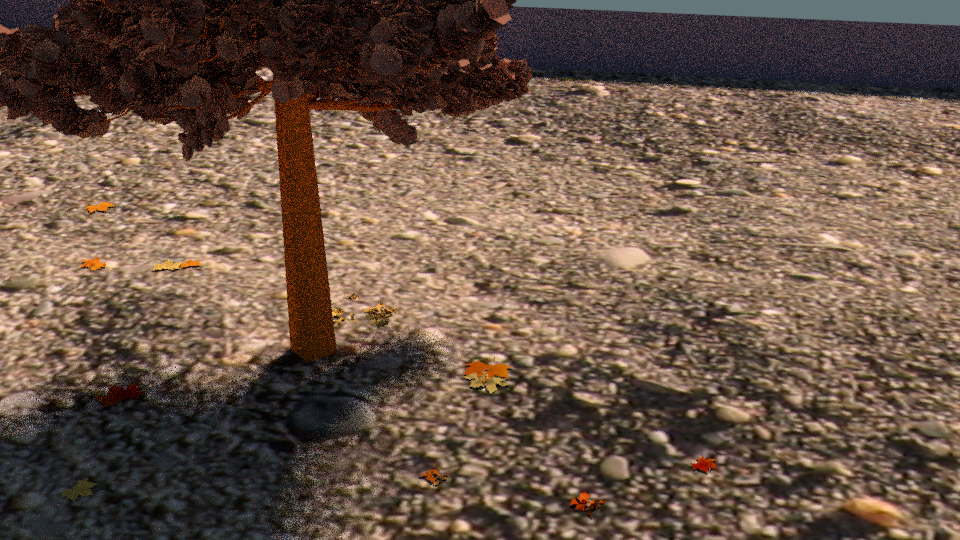
\includegraphics[width=\linewidth]{Figures/GroundDetection_with_ImagePair/im1(1)0001.png}
                \caption{Source image}
                \label{fig:GPSource}
        \end{subfigure}%
        \begin{subfigure}[b]{0.35\textwidth}
        		\centering
                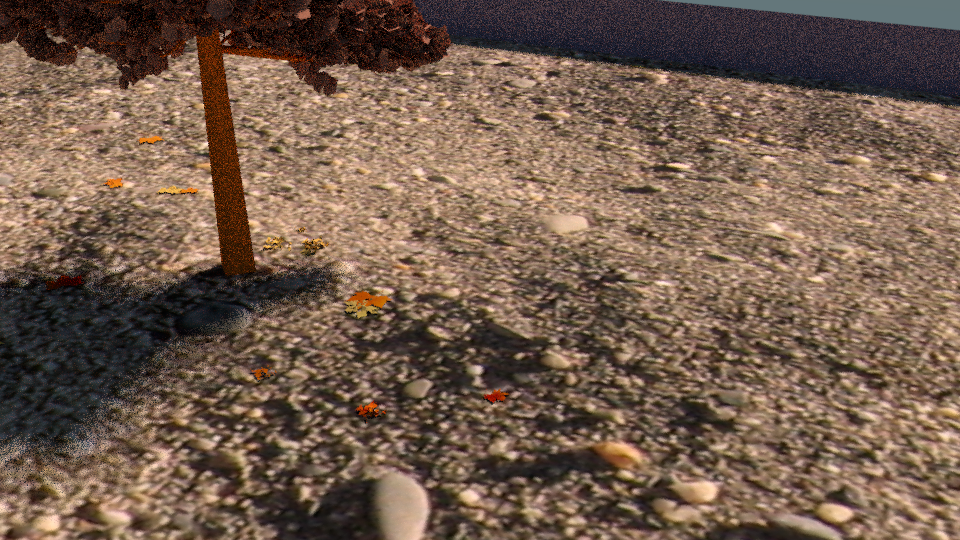
\includegraphics[width=\linewidth]{Figures/GroundDetection_with_ImagePair/im1(2)0001.png}
                \caption{Destination image}
                \label{fig:GPDest}
        \end{subfigure}%
        
        \begin{subfigure}[b]{0.35\textwidth}
                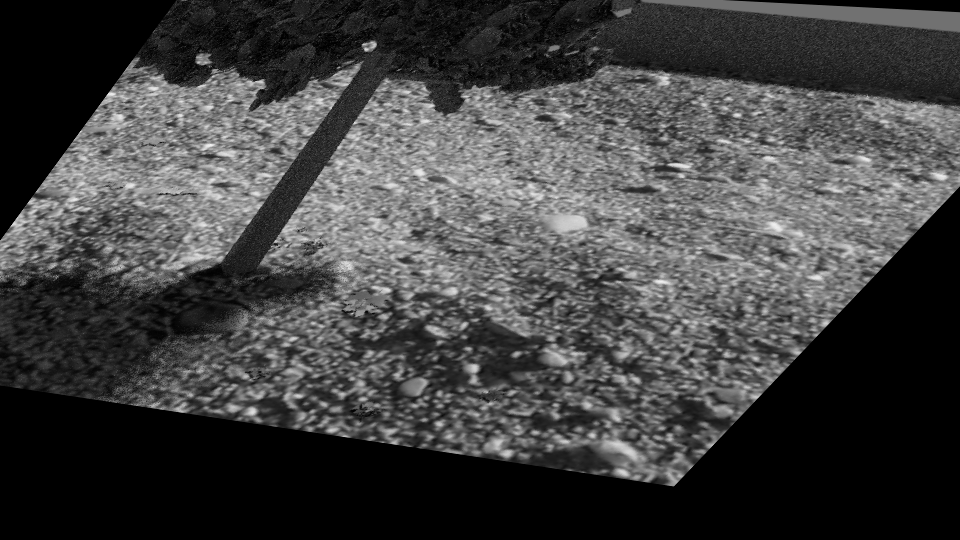
\includegraphics[width=\linewidth]{Figures/GroundDetection_with_ImagePair/im1(2)_step1_warped.png}
                \caption{Warped image}
                \label{fig:GPWarp}
        \end{subfigure}%
        \begin{subfigure}[b]{0.35\textwidth}
                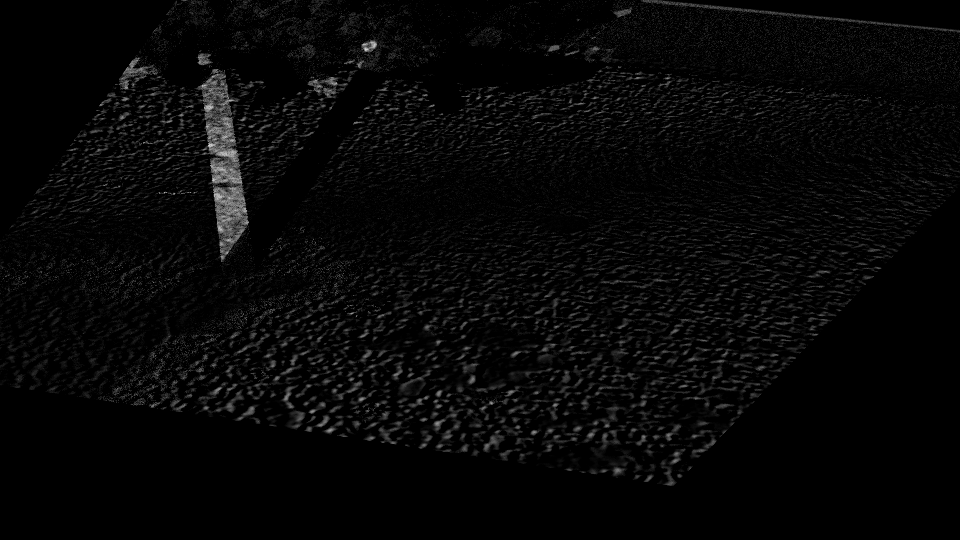
\includegraphics[width=\linewidth]{Figures/GroundDetection_with_ImagePair/im1(2)_step2_subtracted.png}
                \caption{Subtracted image}
                \label{fig:GPSub}
        \end{subfigure}%
        
        \begin{subfigure}[b]{0.35\textwidth}
                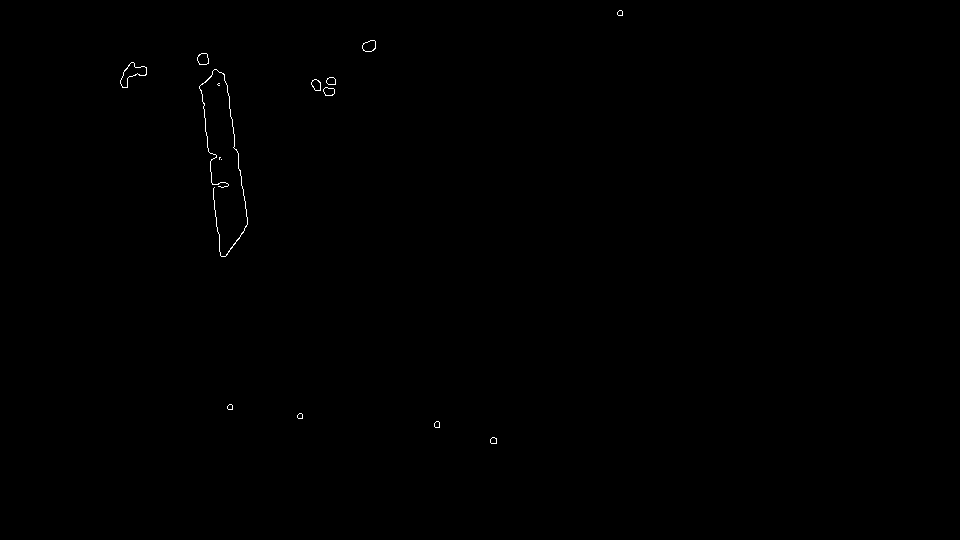
\includegraphics[width=\linewidth]{Figures/GroundDetection_with_ImagePair/im1(2)_step3_2_filters.png}
                \caption{Resulting image from filter pipeline}
                \label{fig:Thresh05ColIm}
        \end{subfigure}
        \begin{subfigure}[b]{0.35\textwidth}
                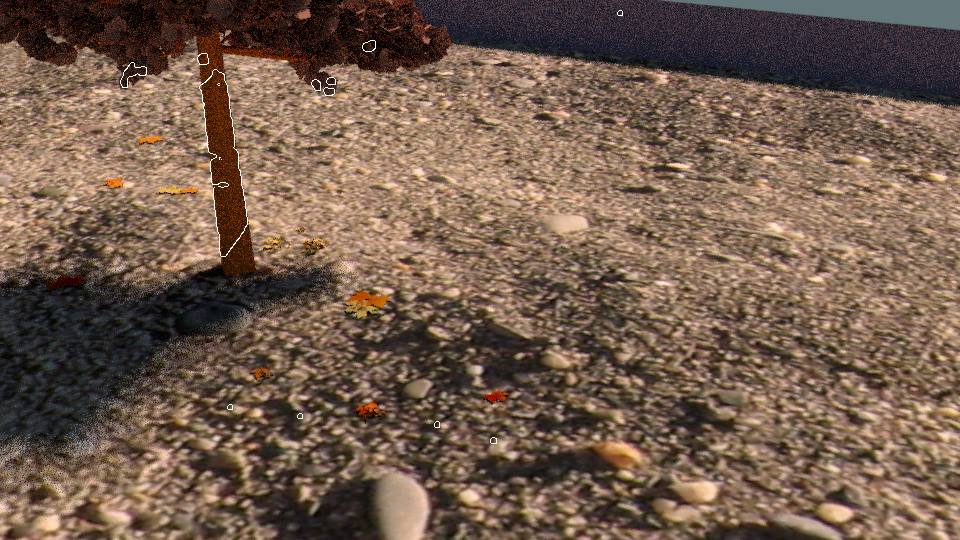
\includegraphics[width=\linewidth]{Figures/GroundDetection_with_ImagePair/im1(2)_step4_detected_not_ground.png}
                \caption{Resulting image overlaid with Destination image}
                \label{fig:GPOverlay}
        \end{subfigure}
        
        \begin{subfigure}[b]{0.7\textwidth}
                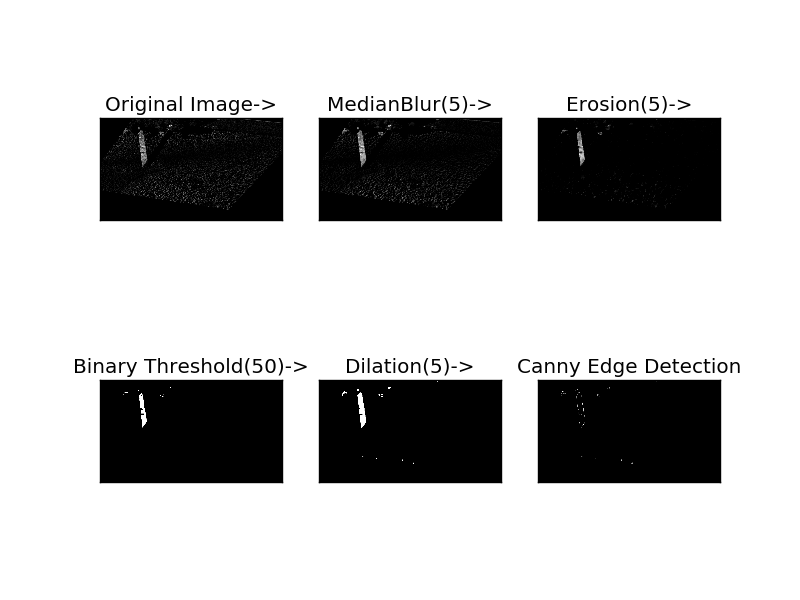
\includegraphics[width=\linewidth]
                {{Figures/GroundDetection_with_ImagePair/im1(2)_step3_1_filters.png}}
                \caption{Filters applied to ground plane detection results.}
                \label{fig:GroundPlFilt}
        \end{subfigure}
        \caption{Overview of ground plane detection algorithm.}\label{fig:GroundPl}
\end{figure*}


\begin{figure*}
        \begin{subfigure}[b]{0.5\textwidth}
                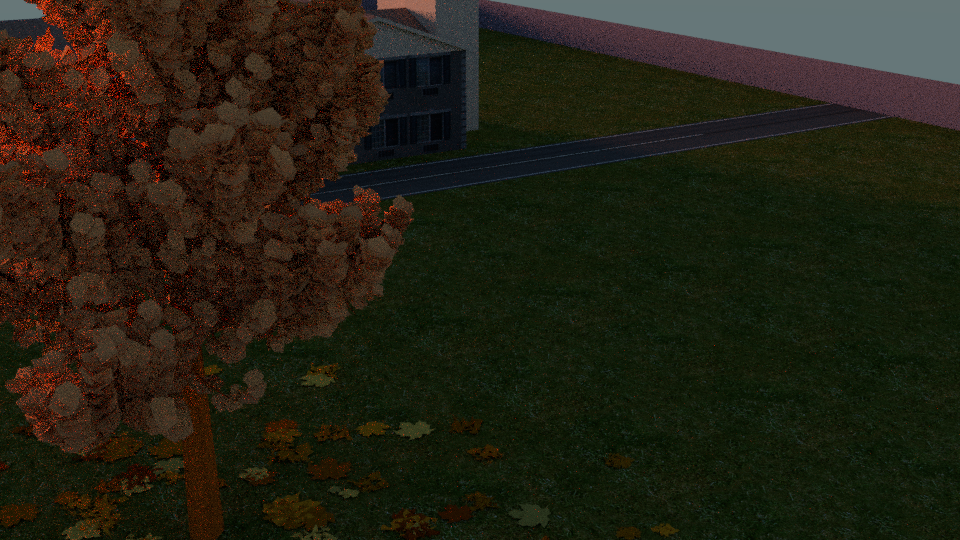
\includegraphics[width=\linewidth]{Figures/ColorFigures/im20001.png}
                \caption{Original image}
                \label{fig:ColIm}
        \end{subfigure}%
        \begin{subfigure}[b]{0.5\textwidth}
                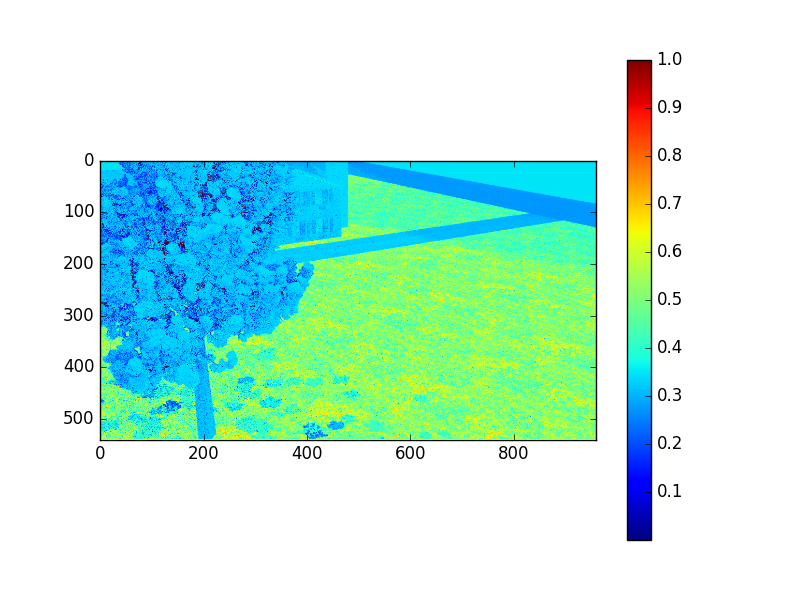
\includegraphics[width=\linewidth]{Figures/ColorFigures/res1_2.png}
                \caption{Normalized g values}
                \label{fig:NormrColIm2}
        \end{subfigure}%
        
        \begin{subfigure}[b]{0.5\textwidth}
                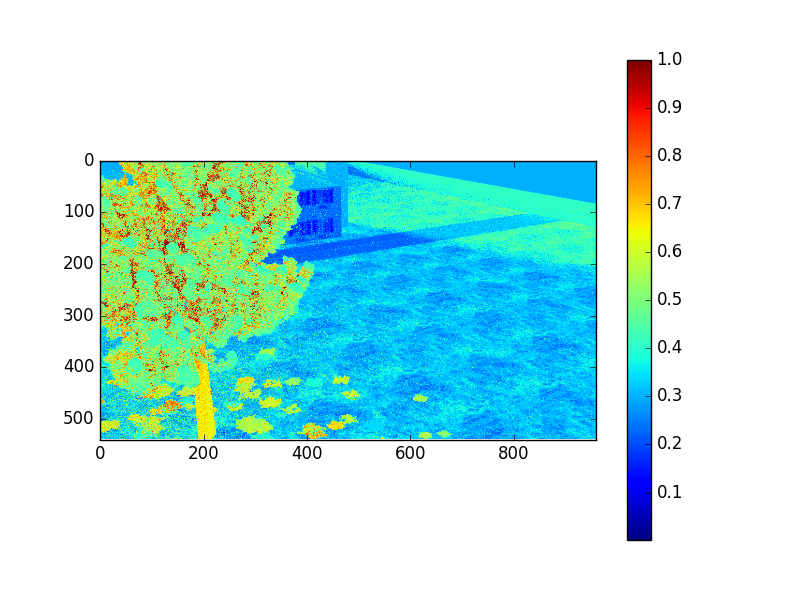
\includegraphics[width=\linewidth]{Figures/ColorFigures/res1.png}
                \caption{Normalized r values}
                \label{fig:NormrColIm}
        \end{subfigure}%
        \begin{subfigure}[b]{0.5\textwidth}
                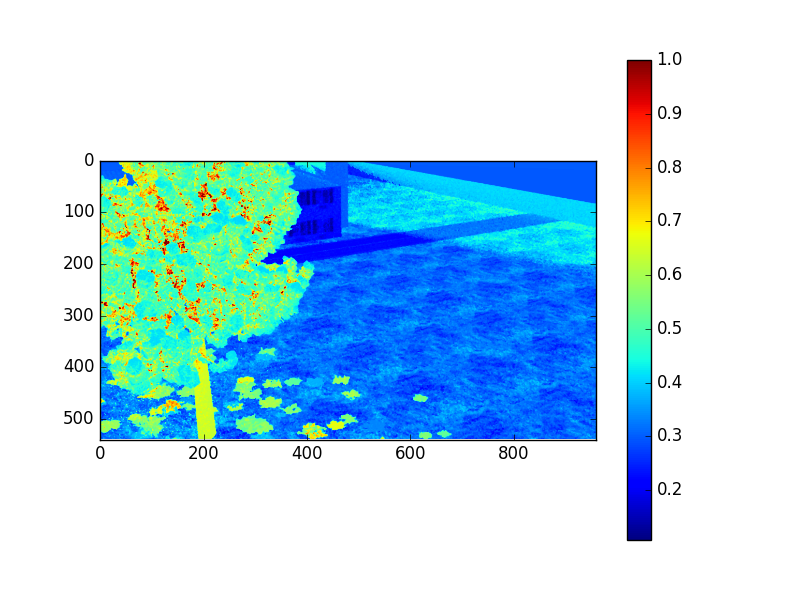
\includegraphics[width=\linewidth]{Figures/ColorFigures/res2.png}
                \caption{Median filter}
                \label{fig:MedFIlColIm}
        \end{subfigure}%
        
        \begin{subfigure}[b]{0.5\textwidth}
                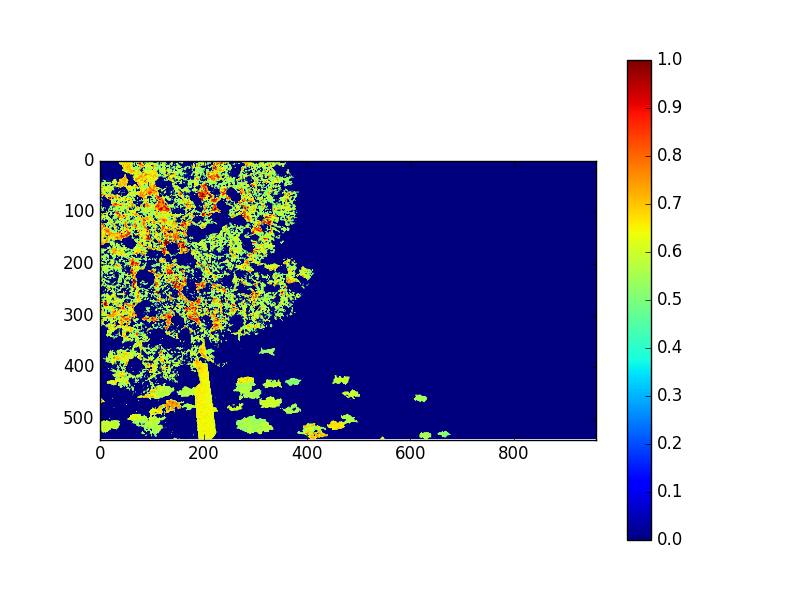
\includegraphics[width=\linewidth]{Figures/ColorFigures/res3_05.png}
                \caption{Resulting image threshold 0.5}
                \label{fig:Thresh05ColIm}
        \end{subfigure}
        \begin{subfigure}[b]{0.5\textwidth}
                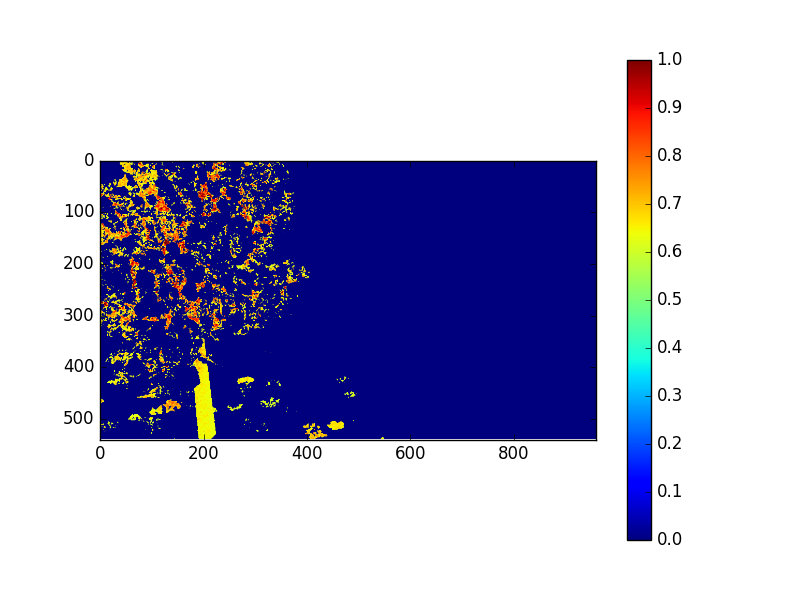
\includegraphics[width=\linewidth]{Figures/ColorFigures/res3_06.png}
                \caption{Resulting image threshold 0.6}
                \label{fig:Thresh05ColIm}
        \end{subfigure}
        \caption{Overview of foliage color filtering.}\label{fig:ColFilters}
\end{figure*}

\begin{figure*}
        \begin{subfigure}[b]{0.3\textwidth}
                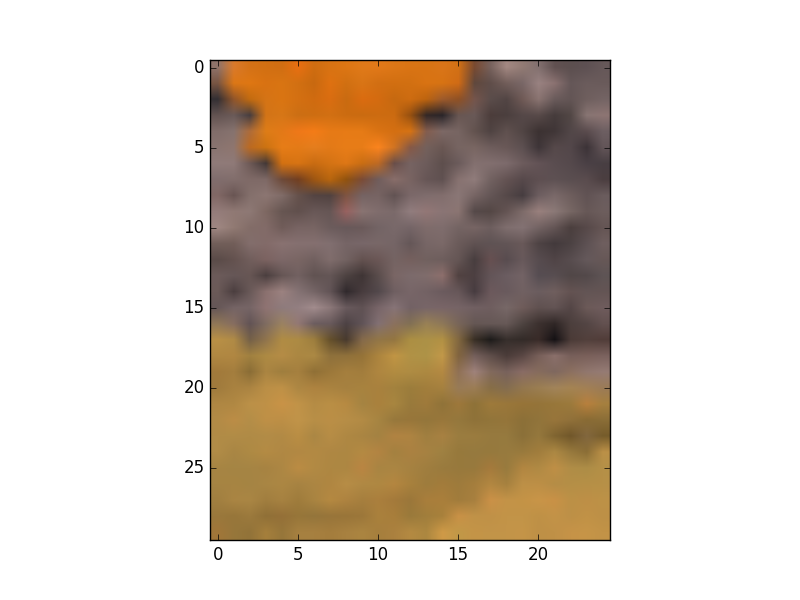
\includegraphics[width=\linewidth]{Figures/EdgeFigures/TileColor.png}
                \caption{Color tile}
                \label{fig:ColTile}
        \end{subfigure}%
        \begin{subfigure}[b]{0.3\textwidth}
                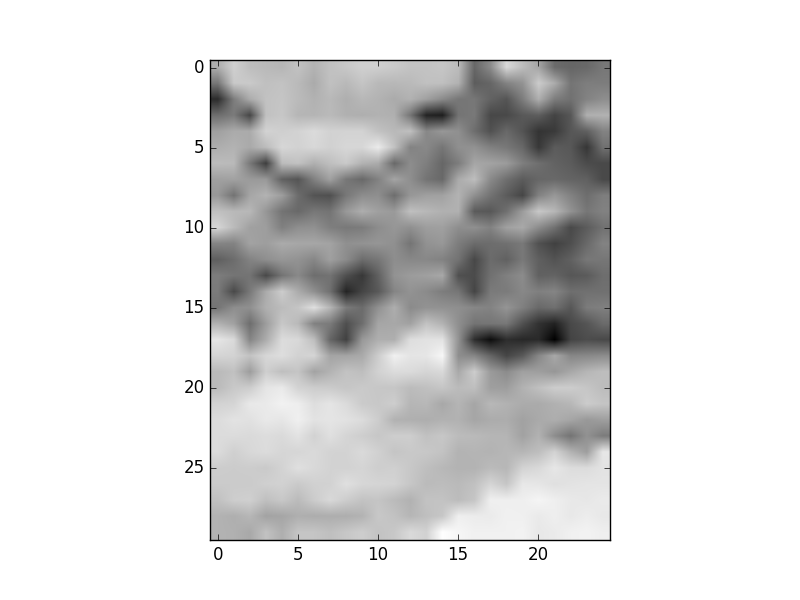
\includegraphics[width=\linewidth]{Figures/EdgeFigures/TileGray.png}
                \caption{Grayscale tile}
                \label{fig:GrayTile}
        \end{subfigure}%
        \begin{subfigure}[b]{0.3\textwidth}
                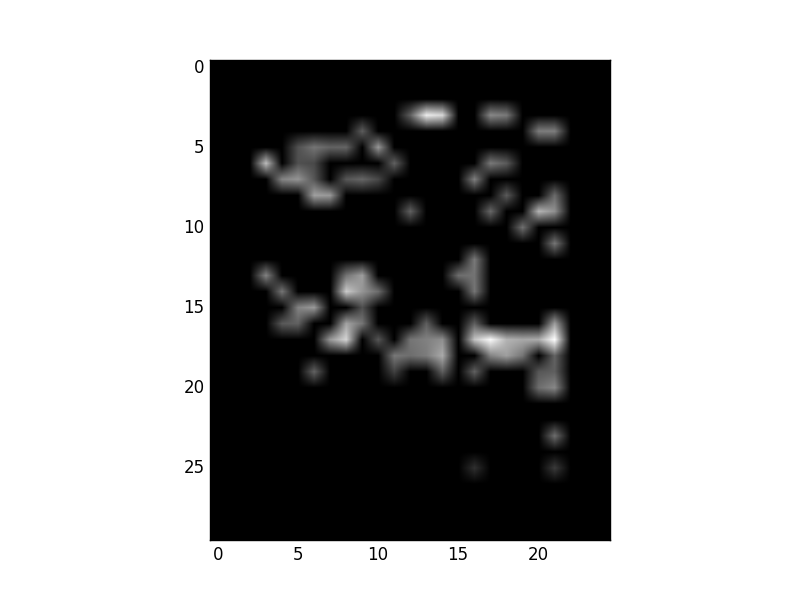
\includegraphics[width=\linewidth]{Figures/EdgeFigures/TileCorner.png}
                \caption{FAST Corner filter tile}
                \label{fig:CornerTile}
        \end{subfigure}%
        
        \begin{subfigure}[b]{0.3\textwidth}
                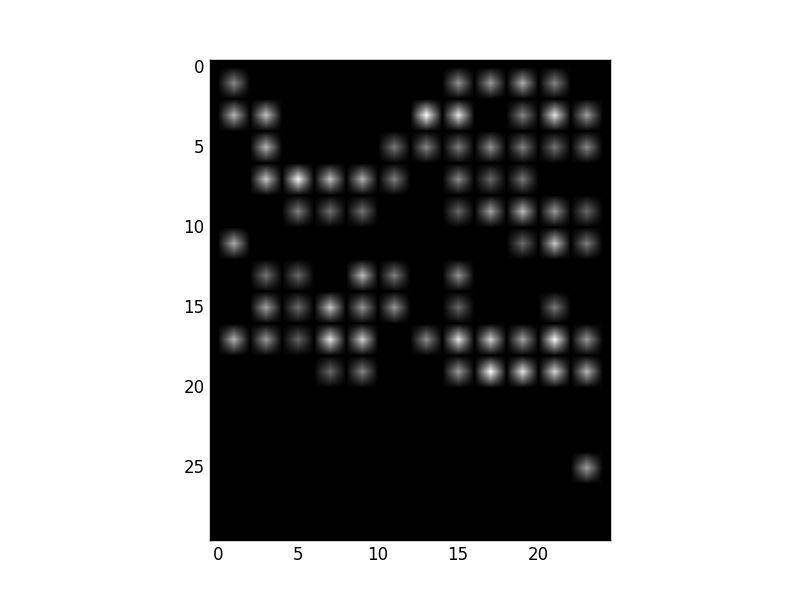
\includegraphics[width=\linewidth]{Figures/EdgeFigures/TileHOG.png}
                \caption{Histogram of Gradients tile}
                \label{fig:HOGTile}
        \end{subfigure}
        \begin{subfigure}[b]{0.3\textwidth}
                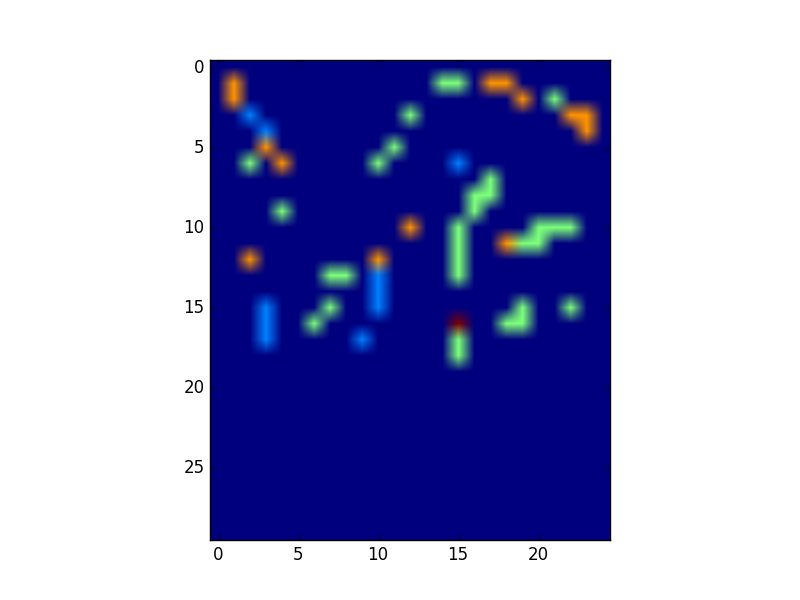
\includegraphics[width=\linewidth]{Figures/EdgeFigures/TileEdgeOrient.png}
                \caption{Maximal edge orientation tile}
                \label{fig:EdgeOrientTile}
        \end{subfigure}
        \begin{subfigure}[b]{0.3\textwidth}
                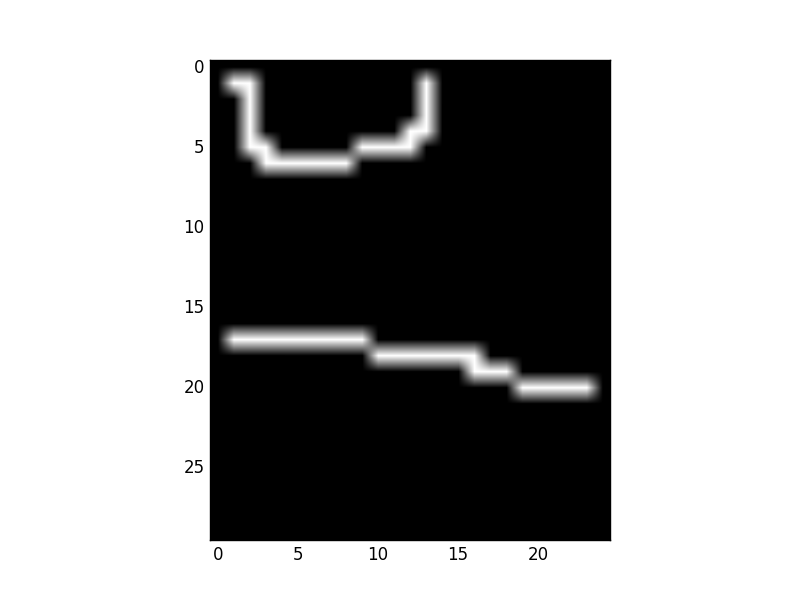
\includegraphics[width=\linewidth]{Figures/EdgeFigures/TileCanny.png}
                \caption{Canny Edge Tile}
                \label{fig:CannyTile}
        \end{subfigure}
        \caption{Overview of edge and corner filters on exemplary leaf sized tile. The color coding in subfigure \ref{fig:EdgeOrientTile} is: dark blue:= horizontal edge, light blue:= vertical edge, green:= $45\degree$ edge, orange:= $135\degree$ edge.}\label{fig:EdgeFilters}
\end{figure*}

\begin{figure*}
        \begin{subfigure}[b]{0.3\textwidth}
                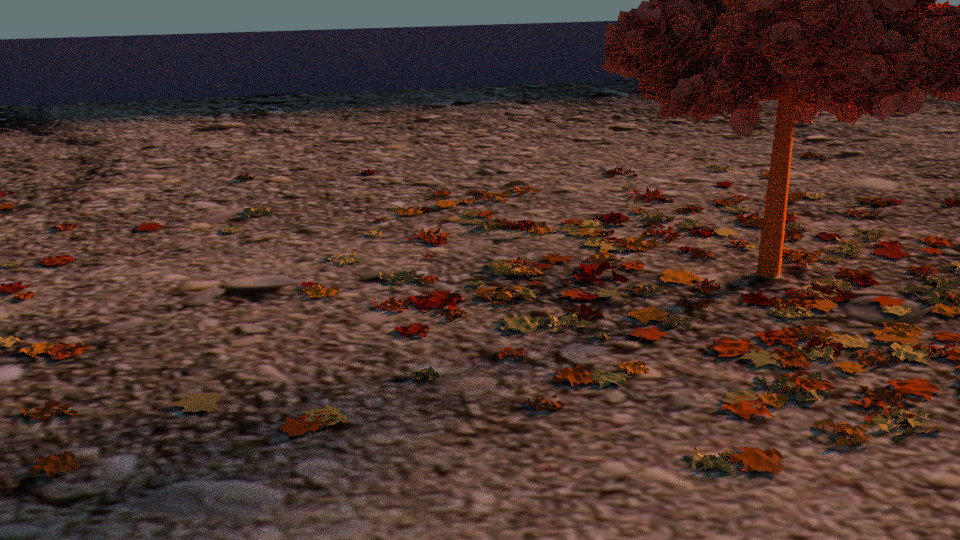
\includegraphics[width=\linewidth]{Figures/Combi/im1(2)0001.png}
                \caption{Orig. Image}
                \label{fig:ResOrigImg}
        \end{subfigure}%
        \begin{subfigure}[b]{0.3\textwidth}
                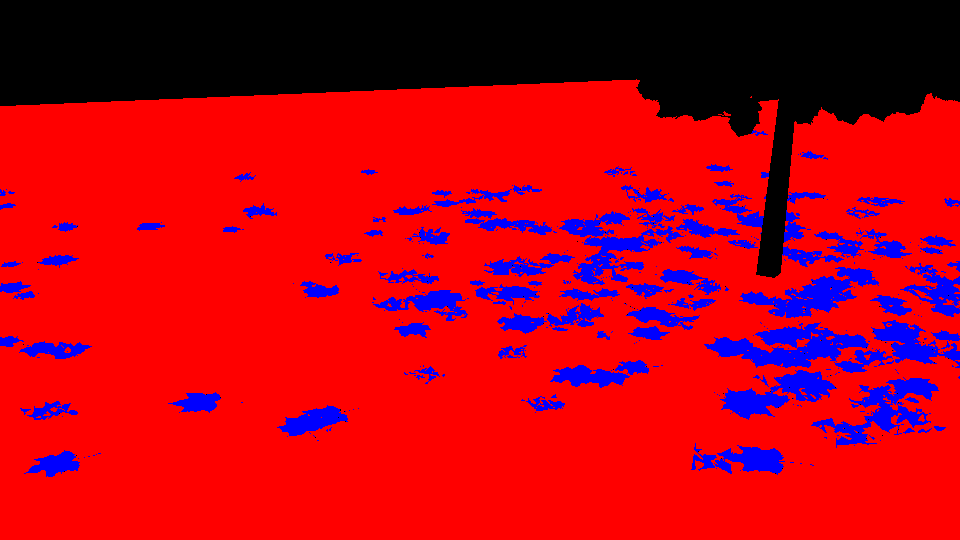
\includegraphics[width=\linewidth]{Figures/Combi/im1(2)_anno0001.png}
                \caption{GT}
                \label{fig:ResGT}
        \end{subfigure}%
        \begin{subfigure}[b]{0.3\textwidth}
                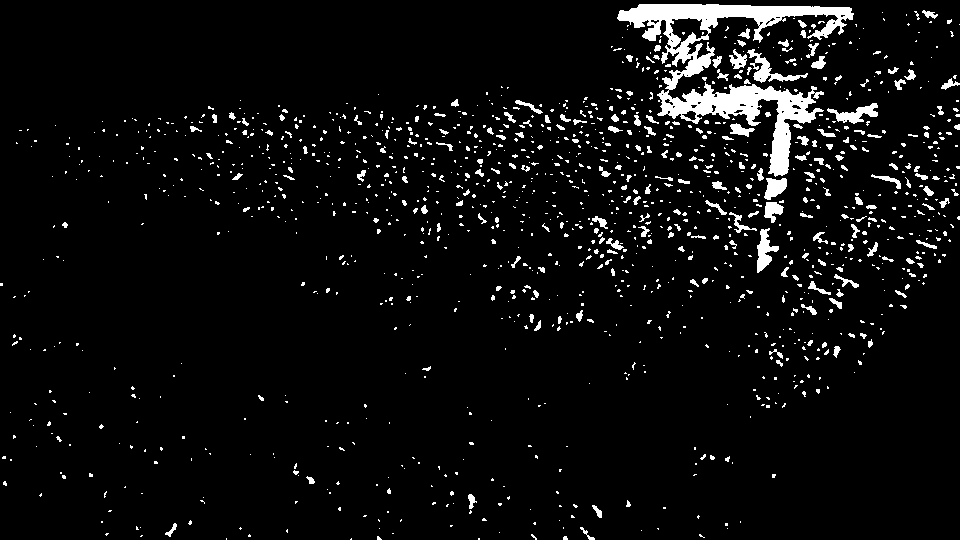
\includegraphics[width=\linewidth]{Figures/Combi/im1(2)_step3_otsus_threshold.png}
                \caption{Ground detection}
                \label{fig:ResGD}
        \end{subfigure}%
        
        \begin{subfigure}[b]{0.3\textwidth}
                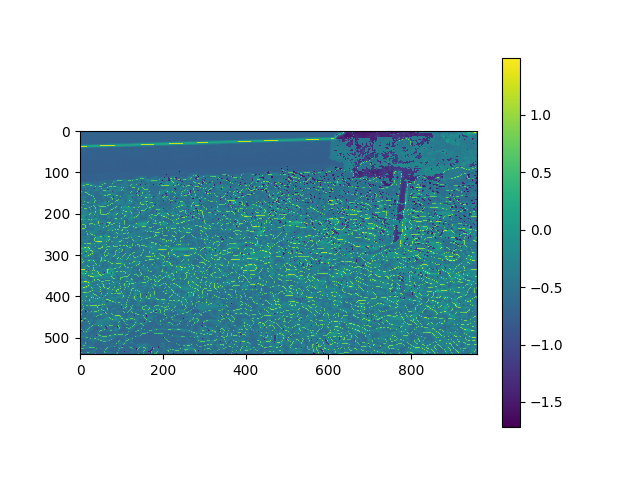
\includegraphics[width=\linewidth]{Figures/Combi/res1.png}
                \caption{inverted GD + color + edges + corner}
                \label{fig:ResSum}
        \end{subfigure}
        \begin{subfigure}[b]{0.3\textwidth}
                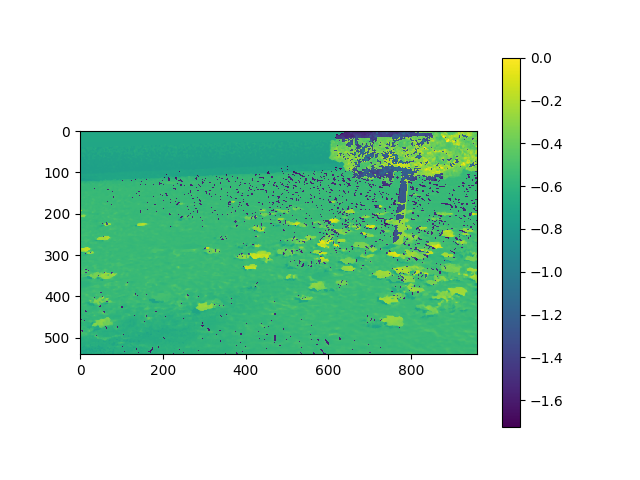
\includegraphics[width=\linewidth]{Figures/Combi/res2.png}
                \caption{inverted GD + color}
                \label{fig:ResColor}
        \end{subfigure}
        \begin{subfigure}[b]{0.3\textwidth}
                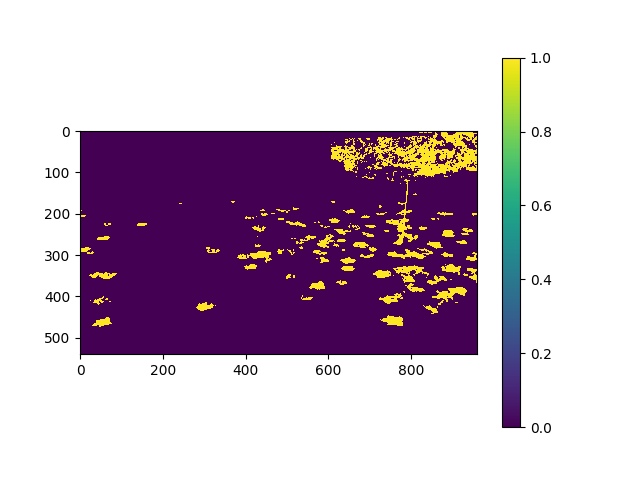
\includegraphics[width=\linewidth]{Figures/Combi/res3.png}
                \caption{thresholded, thr=-0.4}
                \label{fig:CannyTile}
        \end{subfigure}
        \caption{Example for the combination of filters}
	 \label{fig:Res}
\end{figure*}

\newpage
%----------------------------------------------------------------------------------------
%	REFERENCE LIST
%----------------------------------------------------------------------------------------
\phantomsection
\bibliographystyle{unsrt}
\bibliography{sample}

%----------------------------------------------------------------------------------------

\end{document}
